\section{Implementierung}

\subsection{Back-End}

\subsubsection{Datenmodelle}

\subsubsection{Datenstore}

\subsection{Front-End}

Nachfolgend wir die Implementierung der GUI beschrieben. Da einige Komponenten schon existiert haben und für den Editor nicht extra

\subsubsection{ShortcutField}

\subsubsection{Accordion}

\newpage

\subsubsection{Check-Button}

Zur Implementierung des im Abschnitt (XXX) erwähnten Check-Buttons wurde zunächst das Interface ICheckComponent erstellt. Indessen wird die Grundfunktionalität einer CheckComponent definiert. Diese besteht darin, dass der Checked-Zustand gesetzt (setChecked(...)) und gelesen (isChecked()) werden kann. Außerdem informiert ein Listener über Änderungen des Zustands. Wird Checked auf true gesetzt, so soll innerhalb der Komponente ein grüner Hacken andernfalls ein rotes Kreuz angezeigt werden. 

Die Klasse CheckToggleButton implementiert das beschriebene Interface und erbt von der Swing Klasse JToggleButton. Sie kümmert sich um das Einfügen und Aktualisieren des richtigen Symbols. Innerhalb von setChecked(...) wird die private Methode \_updateIcon() aufgerufen, welche ihrerseits das jeweilige Symbol über das gesetzte Icon zeichnet (Siehe Anhang (XXX)). Insgesamt stellt ein CheckToggleButton eine vollwertige CheckComponent dar, welche direkt verwendet werden kann.

\begin{figure}[H]
	\centering
	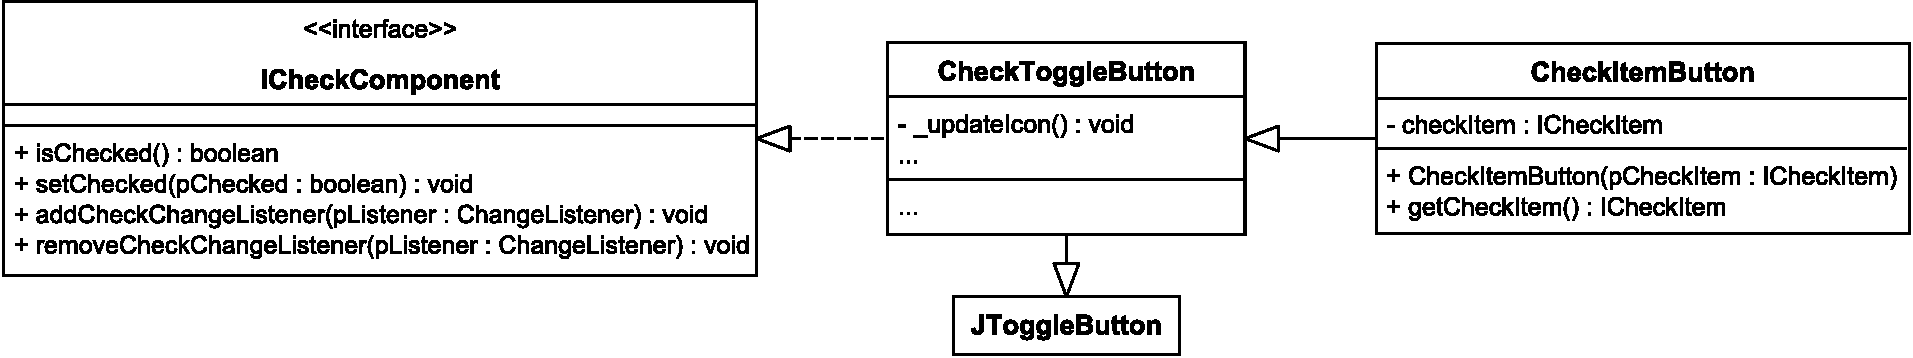
\includegraphics[width=1\linewidth]{../graphic/diagrams/CD_CheckButton/CD_CheckButton}
	\caption{Klassendiagramm des CheckButtons}
	\label{fig:cdcheckbutton}
\end{figure}

Um die Benutzung von CheckToggleButtons innerhalb des Shortcut Editors einfacher zu gestalten, wurde die Klasse CheckItemButton eingeführt, welche CheckToggleButton erweitet und über den Konstruktor ein ICheckItem (siehe (XXX)) aufnehmen kann. Innerhalb dieses Konstruktors werden dem Button alle Eigenschaften entsprechend dem ICheckItem gesetzt (z.B. Checked-Zustand oder Icon).

\subsubsection{CheckItemContainer}

\begin{wrapfigure}[13]{r}[0cm]{160px}
	\vspace{-12px}
	\centering
	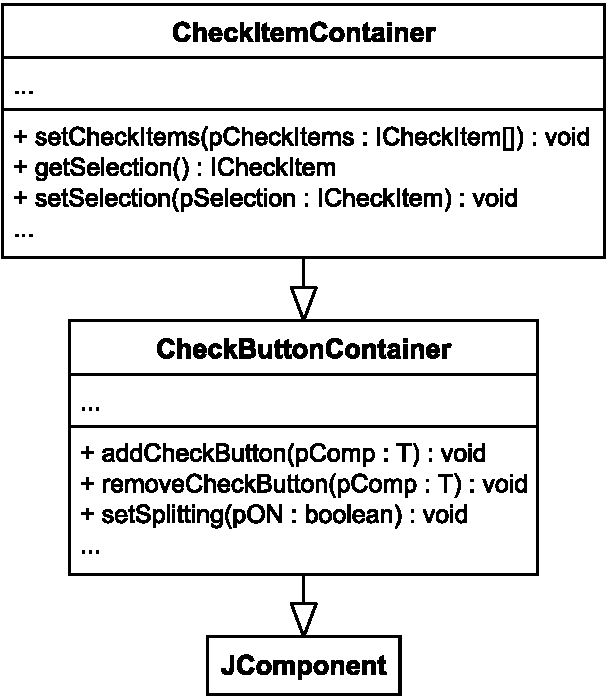
\includegraphics[width=.95\linewidth]{../graphic/diagrams/CD_CheckItemContainer/CD_CheckItemContainer}
	\caption{}
	\label{fig:cdcheckitemcontainer}
\end{wrapfigure}

ewrfqeochwre uow eufoiwqfqjwdeifj iewdj qoew oqwi hequwhe gqweiughqw iuuihqweughfqwueihf  eihwquifh qrhe gfuiqwueihf quih qwihegfuhqwui heuih wqwihe uiqhwueihfquiw hqwheui fhquiwhe fuhweewuhwquei hfhwr fuiqhw 

ewrfqeochwre uow eufoiwqfqjwdeifj iewdj qoew oqwi hequwhe gqweiughqw iuuihqweughfqwueihf  eihwquifh qrhe gfuiqwueihf quih qwihegfuhqwui heuih wqwihe uiqhwueihfquiw hqwheui fhquiwhe fuhweewuhwquei hfhwr fuiqhw 

ewrfqeochwre uow eufoiwqfqjwdeifj iewdj qoew oqwi hequwhe gqweiughqw iuuihqweughfqwueihf  eihwquifh qrhe gfuiqwueihf quih qwihegfuhqwui heuih wqwihe uiqhwueihfquiw hqwheui fhquiwhe fuhweewuhwquei hfhwr fuiqhw 

ewrfqeochwre uow eufoiwqfqjwdeifj iewdj qoew oqwi hequwhe gqweiughqw iuuihqweughfqwueihf  eihwquifh qrhe gfuiqwueihf quih qwihegfuhqwui heuih wqwihe uiqhwueihfquiw hqwheui fhquiwhe fuhweewuhwquei hfhwr fuiqhw 

\newpage